\documentclass[
    xcolor={svgnames,dvipsnames},
    hyperref={colorlinks, citecolor=DeepPink4, linkcolor=DarkRed, urlcolor=DarkBlue}
    ]{beamer}  % for hardcopy add 'trans'

\mode<presentation>
{
  \usetheme{Singapore}
  % or ...
  \setbeamercovered{transparent}
  % or whatever (possibly just delete it)
}



\addtobeamertemplate{navigation symbols}{}{%
    \usebeamerfont{footline}%
    \usebeamercolor[fg]{footline}%
    \hspace{1em}%
    \insertframenumber/\inserttotalframenumber
}



\usepackage{fontspec} 
%\usepackage[xcharter]{newtxmath}
%\setmainfont{XCharter}
\usepackage{unicode-math}
%\setmathfont{XCharter-Math.otf}
\setmonofont{DejaVu Sans Mono}[Scale=MatchLowercase] % provides unicode characters 

\usepackage{tikz}
\usetikzlibrary{matrix, shapes, arrows.meta, positioning, fit, backgrounds, calc}

% \usetikzlibrary{matrix, arrows.meta, positioning, calc, backgrounds}

% for tikz
\usepackage{pgfplots}
\usepgfplotslibrary{fillbetween}
\pgfplotsset{compat=1.16}

\usepackage{varwidth}
\usepackage{minted}
\usemintedstyle{friendly}
\setminted[python]{
  fontsize=\small,
  baselinestretch=1.2,
  bgcolor=codebg,
  linenos=false,
  breaklines=true,
  frame=none
}
\setminted[matlab]{
  fontsize=\small,
  baselinestretch=1.2,
  bgcolor=codebg,
  linenos=false,
  breaklines=true,
  frame=none
}
\setminted[julia]{
  fontsize=\small,
  baselinestretch=1.2,
  bgcolor=codebg,
  linenos=false,
  breaklines=true,
  frame=none
}
%\setminted{mathescape, frame=lines, framesep=3mm}
%\newminted{python}{}
%\newminted{c}{mathescape,frame=lines,framesep=4mm,bgcolor=bg}
%\newminted{java}{mathescape,frame=lines,framesep=4mm,bgcolor=bg}
%\newminted{julia}{mathescape,frame=lines,framesep=4mm,bgcolor=bg}
%\newminted{ipython}{mathescape,frame=lines,framesep=4mm,bgcolor=bg}

\usepackage{graphicx}
\usepackage{amsmath, amssymb, amsthm}
\usepackage{bbm}
\usepackage{mathrsfs}
\usepackage{xcolor}
\usepackage{fancyvrb}


% Quotes at start of chapters / sections
\usepackage{epigraph}  
\renewcommand{\epigraphwidth}{6in}

%% Fonts

%\usepackage[T1]{fontenc}
\usepackage{mathpazo}
%\usepackage{fontspec}
%\defaultfontfeatures{Ligatures=TeX}
%\setsansfont[Scale=MatchLowercase]{DejaVu Sans}
%\setmonofont[Scale=MatchLowercase]{DejaVu Sans Mono}
%\setmathfont{Asana Math}
%\setmainfont{Optima}
%\setmathrm{Optima}
%\setboldmathrm[BoldFont={Optima ExtraBlack}]{Optima Bold}

% Some colors

\definecolor{containerblue}{RGB}{66, 133, 244}
\definecolor{leafgreen}{RGB}{52, 168, 83}
\definecolor{textgray}{RGB}{51, 51, 51}
\definecolor{backgroundgray}{RGB}{248, 249, 250}
\definecolor{codebg}{RGB}{241, 241, 241}
\definecolor{aquamarine}{RGB}{69,139,116}
\definecolor{midnightblue}{RGB}{25,25,112}
\definecolor{darkslategrey}{RGB}{47,79,79}
\definecolor{darkorange4}{RGB}{139,90,0}
\definecolor{dogerblue}{RGB}{24,116,205}
\definecolor{blue2}{RGB}{0,0,238}
\definecolor{bg}{rgb}{0.95,0.95,0.95}
\definecolor{DarkOrange1}{RGB}{255,127,0}
\definecolor{ForestGreen}{RGB}{34,139,34}
\definecolor{DarkRed}{RGB}{139, 0, 0}
\definecolor{DarkBlue}{RGB}{0, 0, 139}
\definecolor{Blue}{RGB}{0, 0, 255}
\definecolor{Brown}{RGB}{165,42,42}


\setlength{\parskip}{1.5ex plus0.5ex minus0.5ex}

%\renewcommand{\baselinestretch}{1.05}
%\setlength{\parskip}{1.5ex plus0.5ex minus0.5ex}
%\setlength{\parindent}{0pt}

% Typesetting code
\definecolor{bg}{rgb}{0.95,0.95,0.95}
\newcommand{\Fact}{\textcolor{Brown}{\bf Fact. }}
\newcommand{\Facts}{\textcolor{Brown}{\bf Facts }}
\newcommand{\keya}{\textcolor{turquois4}{\bf Key Idea. }}
\newcommand{\Factnodot}{\textcolor{Brown}{\bf Fact }}
\newcommand{\Eg}{\textcolor{ForestGreen}{Example. }}
\newcommand{\Egs}{\textcolor{ForestGreen}{Examples. }}
\newcommand{\Ex}{{\bf Ex. }}



\renewcommand{\theFancyVerbLine}{\sffamily
    \textcolor[rgb]{0.5,0.5,1.0}{\scriptsize {\arabic{FancyVerbLine}}}}

\newcommand{\navy}[1]{\textcolor{DarkBlue}{\bf #1}}
\newcommand{\brown}[1]{\textcolor{Brown}{\sf #1}}
\newcommand{\green}[1]{\textcolor{ForestGreen}{\sf #1}}
\newcommand{\blue}[1]{\textcolor{Blue}{\sf #1}}
\newcommand{\emp}[1]{\textcolor{DarkOrange1}{\bf #1}}
\newcommand{\red}[1]{\textcolor{Red}{\bf #1}}

% Symbols, redefines, etc.

\newcommand{\code}[1]{\texttt{#1}}

\newcommand{\argmax}{\operatornamewithlimits{argmax}}
\newcommand{\argmin}{\operatornamewithlimits{argmin}}

\DeclareMathOperator{\cl}{cl}
\DeclareMathOperator{\interior}{int}
\DeclareMathOperator{\Prob}{Prob}
\DeclareMathOperator{\determinant}{det}
\DeclareMathOperator{\trace}{trace}
\DeclareMathOperator{\Span}{span}
\DeclareMathOperator{\rank}{rank}
\DeclareMathOperator{\cov}{cov}
\DeclareMathOperator{\corr}{corr}
\DeclareMathOperator{\var}{var}
\DeclareMathOperator{\mse}{mse}
\DeclareMathOperator{\se}{se}
\DeclareMathOperator{\row}{row}
\DeclareMathOperator{\col}{col}
\DeclareMathOperator{\range}{rng}
\DeclareMathOperator{\dimension}{dim}
\DeclareMathOperator{\bias}{bias}


% mics short cuts and symbols
\newcommand{\st}{\ensuremath{\ \mathrm{s.t.}\ }}
\newcommand{\setntn}[2]{ \{ #1 : #2 \} }
\newcommand{\cf}[1]{ \lstinline|#1| }
\newcommand{\fore}{\therefore \quad}
\newcommand{\tod}{\stackrel { d } {\to} }
\newcommand{\toprob}{\stackrel { p } {\to} }
\newcommand{\toms}{\stackrel { ms } {\to} }
\newcommand{\eqdist}{\stackrel {\textrm{ \scriptsize{d} }} {=} }
\newcommand{\iidsim}{\stackrel {\textrm{ {\sc iid }}} {\sim} }
\newcommand{\1}{\mathbbm 1}
\newcommand{\dee}{\,{\rm d}}
\newcommand{\given}{\, | \,}
\newcommand{\la}{\langle}
\newcommand{\ra}{\rangle}

\newcommand{\boldA}{\mathbf A}
\newcommand{\boldB}{\mathbf B}
\newcommand{\boldC}{\mathbf C}
\newcommand{\boldD}{\mathbf D}
\newcommand{\boldM}{\mathbf M}
\newcommand{\boldP}{\mathbf P}
\newcommand{\boldQ}{\mathbf Q}
\newcommand{\boldI}{\mathbf I}
\newcommand{\boldX}{\mathbf X}
\newcommand{\boldY}{\mathbf Y}
\newcommand{\boldZ}{\mathbf Z}

\newcommand{\bSigmaX}{ {\boldsymbol \Sigma_{\hboldbeta}} }
\newcommand{\hbSigmaX}{ \mathbf{\hat \Sigma_{\hboldbeta}} }

\newcommand{\RR}{\mathbbm R}
\newcommand{\NN}{\mathbbm N}
\newcommand{\PP}{\mathbbm P}
\newcommand{\EE}{\mathbbm E \,}
\newcommand{\XX}{\mathbbm X}
\newcommand{\ZZ}{\mathbbm Z}
\newcommand{\QQ}{\mathbbm Q}

\newcommand{\fF}{\mathcal F}
\newcommand{\dD}{\mathcal D}
\newcommand{\lL}{\mathcal L}
\newcommand{\gG}{\mathcal G}
\newcommand{\hH}{\mathcal H}
\newcommand{\nN}{\mathcal N}
\newcommand{\pP}{\mathcal P}




\title{Artificial Neural Networks}

\author{John Stachurski}


\date{2025}


\begin{document}

\begin{frame}
  \titlepage
\end{frame}



\begin{frame}
    \frametitle{Topics}

    \begin{itemize}
        \item History
        \vspace{0.5em}
        \item Computational graphs
        \vspace{0.5em}
        \item Feedforward neural networks
        \vspace{0.5em}
        \item Gradient descent
        \vspace{0.5em}
        \item Why is DL so successful?
        \vspace{0.5em}
    \end{itemize}

\end{frame}


\begin{frame}

    \emp{History}

    \begin{itemize}
        \item 1940s: \brown{McCulloch \& Pitts} create mathematical model of NN
        \vspace{0.5em}
        \item 1950s: \brown{Rosenblatt} develops the perceptron (trainable NN)
        \vspace{0.5em}
        \item 1960s-70s: Limited progress with single layer perceptrons
        \vspace{0.5em}
        \item 1980s: Backpropagation algorithm enables training of MLPs
        \vspace{0.5em}
        \item 1990s: SVMs temporarily overshadow ANNs in popularity
        \vspace{0.5em}
        \item 2000s: Deep learning finds successes in large problems
    \end{itemize}
    
        \vspace{0.5em}
        \vspace{0.5em}
    \emp{Last 10 years:} Explosion of progress in deep learning 

    \begin{itemize}
        \item CNNs, RNNs, LSTMs, transformers, LLMs, etc.
    \end{itemize}

\end{frame}

\begin{frame}{A model of the human brain}
    
    \begin{figure}
       \centering
       \scalebox{0.6}{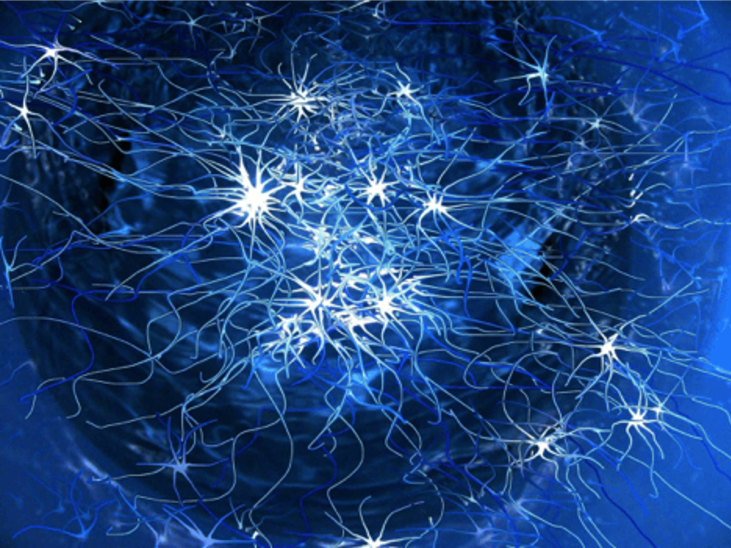
\includegraphics[trim={0cm 0cm 0cm 0cm},clip]{brain.pdf}}
    \end{figure}

    \footnotesize{
    \hspace{5em} -- source: Dartmouth undergraduate journal of science}

\end{frame}


\begin{frame}{A mathematical representation: directed acyclic graph}
    
    \begin{figure}
       \centering
       \scalebox{0.24}{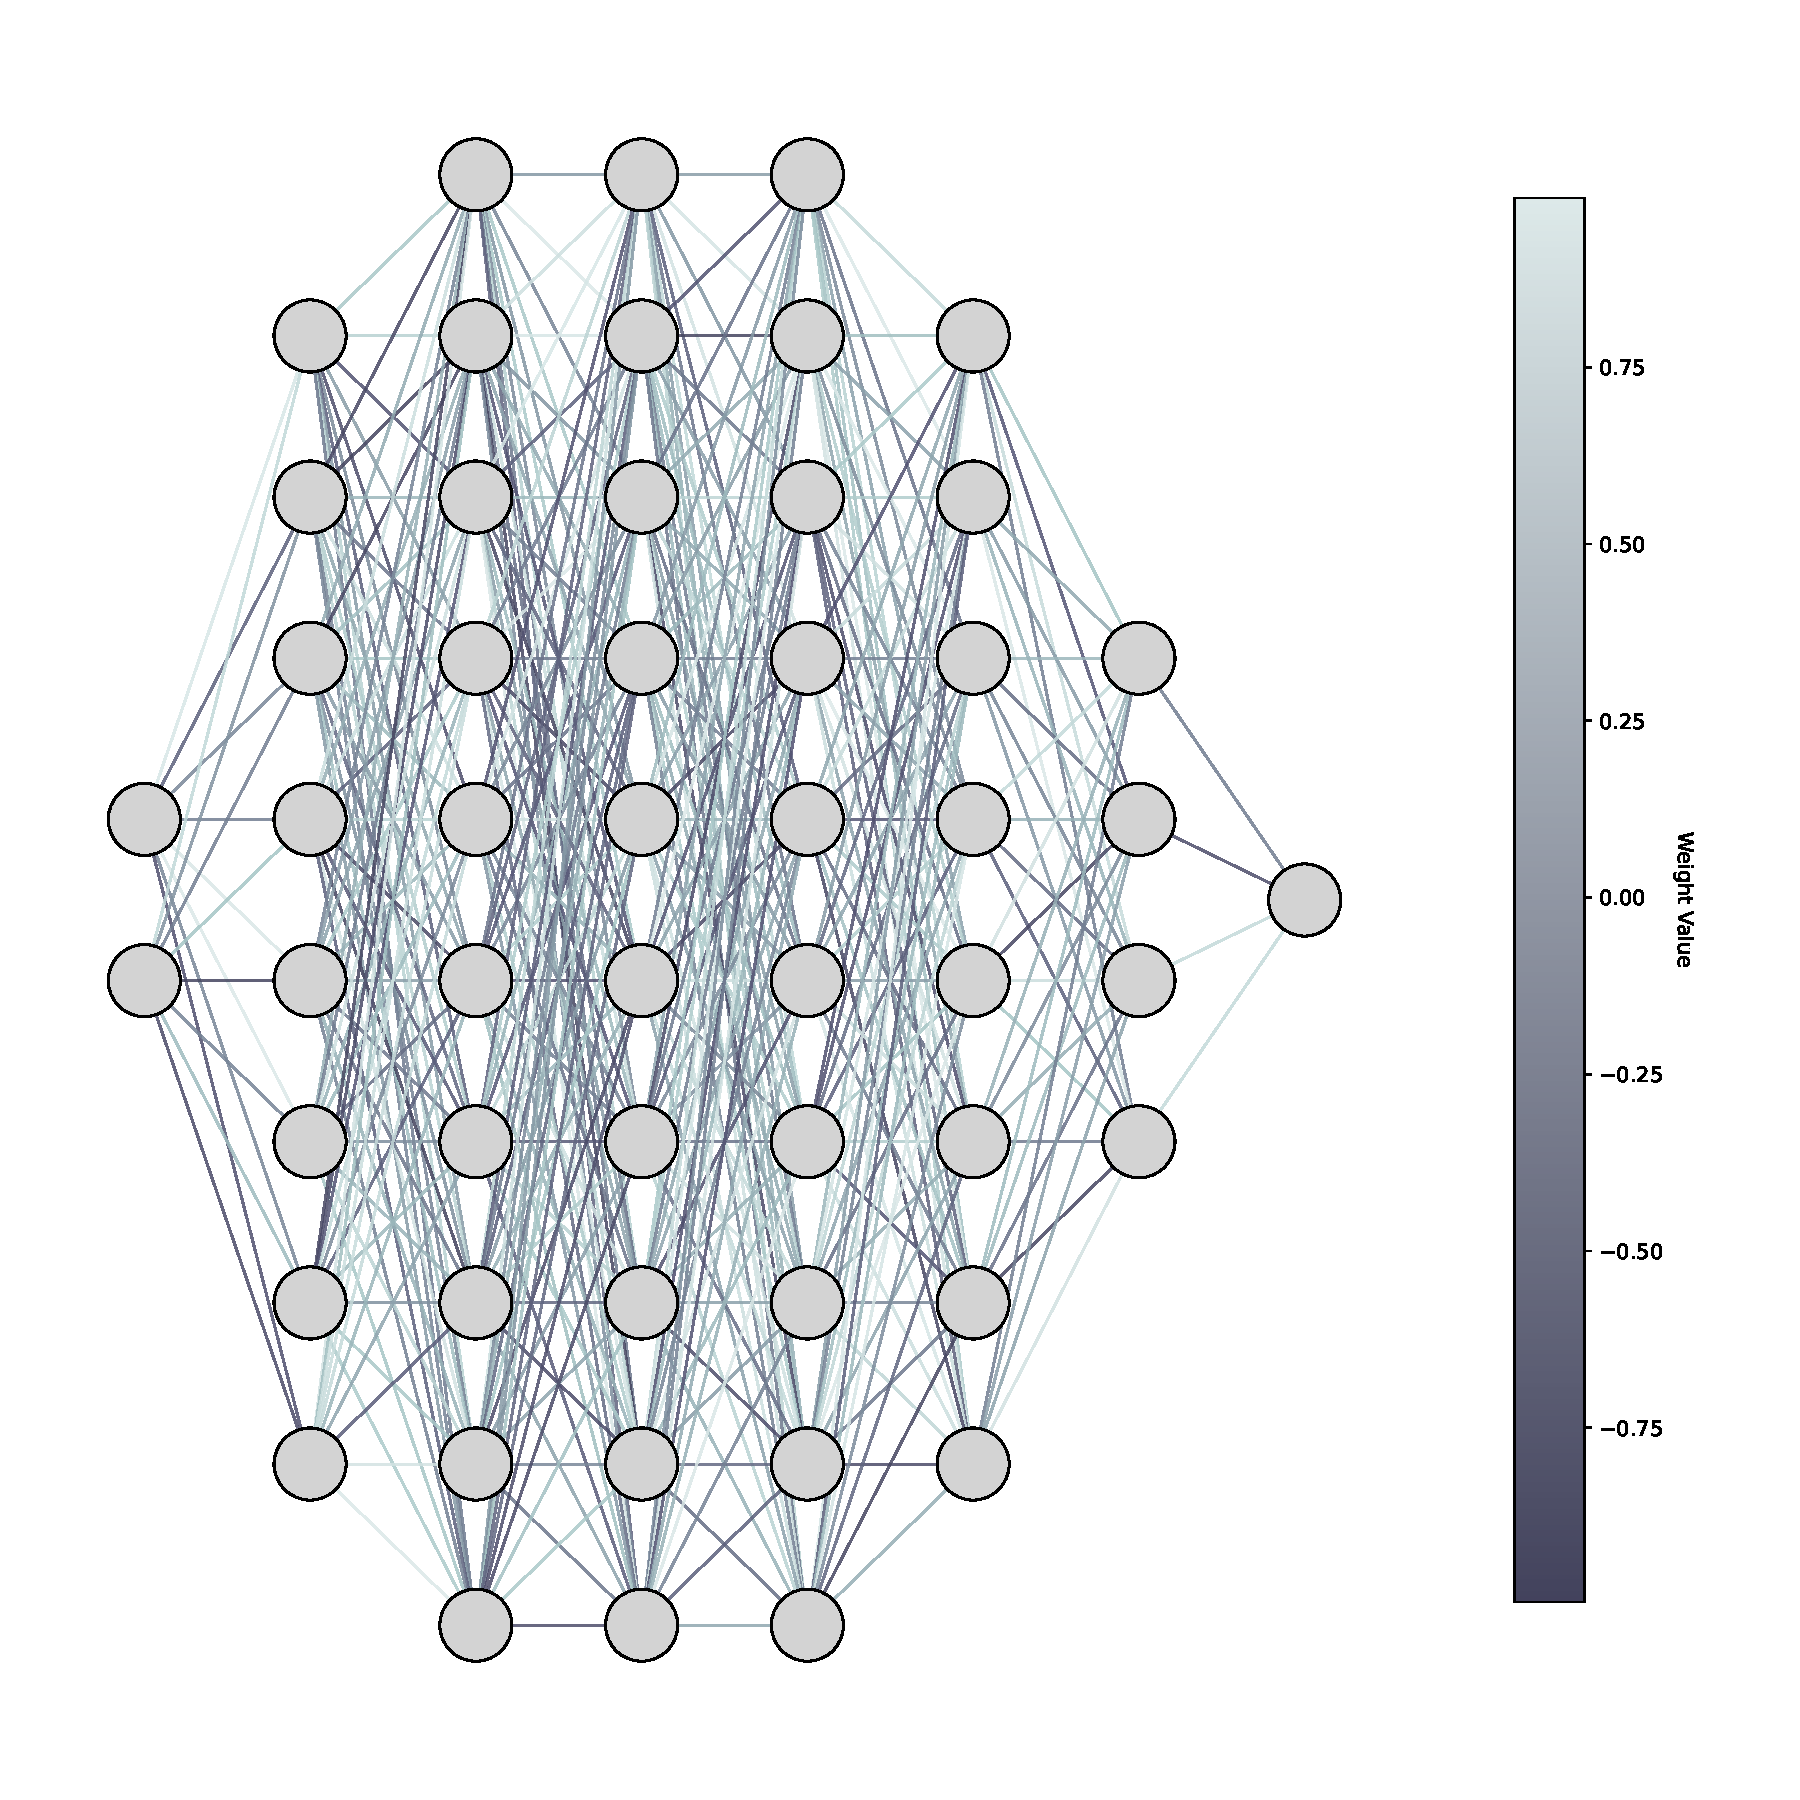
\includegraphics[trim={0cm 0cm 0cm 0cm},clip]{graph.pdf}}
    \end{figure}

\end{frame}


     
\begin{frame}
    
    \begin{tikzpicture}[
            neuron/.style={circle, draw=black, fill=white, minimum size=1cm, thick},
            input neuron/.style={neuron, fill=blue!30},
            output neuron/.style={neuron, fill=orange!40},
            strong pos/.style={green!60!black, line width=1.5mm, ->, >=stealth},
            medium pos/.style={green!60!black, line width=1mm, ->, >=stealth},
            weak neg/.style={red!60!black, line width=0.4mm, ->, >=stealth},
            label/.style={font=\small}
        ]

        % Input neurons (left column)
        \node[input neuron] (N1) at (0,3) {$x_1$};
        \node[input neuron] (N2) at (0,0) {$x_2$};
        \node[input neuron] (N3) at (0,-3) {$x_3$};

        % Output neuron (right column)
        \node[output neuron] (N4) at (6,0) {$y_j$};

        
        \node[anchor=south east, font=\normalsize] at (8.5, 2.5) {$w_{ij}$ is called a ``weight''};

        % Connections with weights
        \draw[strong pos] (N1) -- node[label, above, sloped] {$w_{1j} = 0.85$} (N4);
        \draw[weak neg] (N2) -- node[label, above] {$w_{2j} = -0.15$} (N4);
        \draw[medium pos] (N3) -- node[label, below, sloped] {$w_{3j} = 0.50$} (N4);

    \end{tikzpicture}

\end{frame}

\begin{frame}
    
    \begin{tikzpicture}[
            neuron/.style={circle, draw=black, fill=white, minimum size=1cm, thick},
            input neuron/.style={neuron, fill=blue!30},
            output neuron/.style={neuron, fill=orange!40},
            strong pos/.style={green!60!black, line width=1.5mm, ->, >=stealth},
            medium pos/.style={green!60!black, line width=1mm, ->, >=stealth},
            weak neg/.style={red!60!black, line width=0.4mm, ->, >=stealth},
            label/.style={font=\small}
        ]

        % Input neurons (left column)
        \node[input neuron] (N1) at (0,3) {$x_1$};
        \node[input neuron] (N2) at (0,0) {$x_2$};
        \node[input neuron] (N3) at (0,-3) {$x_3$};

        % Output neuron (right column)
        \node[output neuron] (N4) at (6,0) {$y_j$};

        
        \node[anchor=south east, font=\Large] at (10.5, -0.3)
            {$y_j = \sum_i w_{ij} x_i$};

        % Connections with weights
        \draw[strong pos] (N1) -- node[label, above, sloped] {$w_{1j} = 0.85$} (N4);
        \draw[weak neg] (N2) -- node[label, above] {$w_{2j} = -0.15$} (N4);
        \draw[medium pos] (N3) -- node[label, below, sloped] {$w_{3j} = 0.50$} (N4);

    \end{tikzpicture}

\end{frame}

\begin{frame}
    
    % Neural Network with 3 input neurons and 2 output neurons
% To be included in an existing LaTeX document
% Required packages: tikz

\begin{tikzpicture}[
        neuron/.style={circle, draw=black, fill=white, minimum size=1cm, thick},
        input neuron/.style={neuron, fill=blue!30},
        output neuron/.style={neuron, fill=orange!40},
        strong pos/.style={green!60!black, line width=1.5mm, ->, >=stealth},
        medium pos/.style={green!60!black, line width=1mm, ->, >=stealth},
        weak neg/.style={red!60!black, line width=0.4mm, ->, >=stealth},
        label/.style={font=\small}
    ]

    % Input neurons (left column)
    \node[input neuron] (N1) at (0,3) {$x_1$};
    \node[input neuron] (N2) at (0,0) {$x_2$};
    \node[input neuron] (N3) at (0,-3) {$x_3$};

    % Output neurons (right column)
    \node[output neuron] (N5) at (6,2) {$y_1$};
    \node[output neuron] (N4) at (6,-1) {$y_2$};

    % Connections with weights to N4
    \draw[strong pos] (N1) -- node[label, below, sloped] {$w_{12}$} (N4);
    \draw[weak neg] (N2) -- node[label, below] {$w_{22}$} (N4);
    \draw[medium pos] (N3) -- node[label, below, sloped] {$w_{32}$} (N4);

    % Some connections to the new neuron N5
    \draw[medium pos] (N1) -- node[label, above, sloped] {$w_{11}$} (N5);
    \draw[weak neg] (N3) -- node[label, below, sloped, pos=0.3] {$w_{31}$} (N5);

    % Text in bottom right
    \node[anchor=south east, font=\normalsize] at (10, 1.5) {$y_1 = \sum_i w_{i1} x_i$};
    \node[anchor=south east, font=\normalsize] at (10,-1.5) {$y_2 = \sum_i w_{i2} x_i$};
    \node[anchor=south east, font=\Large] at (10,-3.5) {$\implies y = x W$};

\end{tikzpicture}

\end{frame}


\begin{frame}
    
    Note that we are using \emp{row vectors}:  $y = x W$

        \vspace{0.5em}
        \vspace{0.5em}
    This is natural given our notation 

    \begin{itemize}
        \item $w_{ij}$ points from $i$ to $j$
        \vspace{0.5em}
        \item hence $y_j = \sum_i w_{ij} x_i$
        \vspace{0.5em}
        \item hence $y = x W$
    \end{itemize}

        \vspace{0.5em}
    But it also has another advantage \ldots?


\end{frame}


\begin{frame}
    
    % Required packages for the diagram
% Add these to your preamble if not already included
% \usepackage{tikz}
% \usetikzlibrary{arrows.meta, positioning, calc, backgrounds}
% \usepackage{xcolor}

% Row-major vs Column-major storage diagram
  \begin{tikzpicture}[scale=0.9, transform shape]
    % Define styles
    \tikzset{
        cell/.style={
            rectangle, 
            minimum size=1cm, 
            draw=black,
            thick,
            anchor=center
        },
        memory cell/.style={
            rectangle,
            minimum width=1cm,
            minimum height=1cm,
            draw=black,
            thick,
            anchor=center
        },
        arrow style/.style={-{Stealth[scale=1.5]}, thick},
        label style/.style={font=\small\bfseries}
    }
    
    % Row-major memory layout
    \begin{scope}[shift={(0,0)}]
        % 4 CELLS FOR 2x2 MATRIX
        \node[memory cell] (m0) at (0*1.2,0) {$W_{11}$};
        \node[memory cell] (m1) at (1*1.2,0) {$W_{12}$};
        \node[memory cell] (m2) at (2*1.2,0) {$W_{21}$};
        \node[memory cell] (m3) at (3*1.2,0) {$W_{22}$};
        
        % Highlight rows in row-major
        \begin{scope}[on background layer]
            \fill[red!10] ($(m0) + (-0.6,-0.6)$) rectangle ($(m1) + (0.6,0.6)$);
            \fill[blue!10] ($(m2) + (-0.6,-0.6)$) rectangle ($(m3) + (0.6,0.6)$);
        \end{scope}
        
        % Label to the right
        \node[right=0.8cm of m3, font=\large\bfseries] {row-major storage};
    \end{scope}
    
    % Matrix definition - POSITIONED IN THE MIDDLE and using manual positioning
    \begin{scope}[shift={(0,-3.5)}]
        % Create matrix W manually without the matrix library
        \node[cell] (W11) at (0,0) {$W_{11}$};
        \node[cell] (W12) at (1,0) {$W_{12}$};
        \node[cell] (W21) at (0,-1) {$W_{21}$};
        \node[cell] (W22) at (1,-1) {$W_{22}$};
    \end{scope}
    
    % Column-major memory layout
    \begin{scope}[shift={(0,-7)}]
        % 4 CELLS FOR 2x2 MATRIX
        \node[memory cell] (c0) at (0*1.2,0) {$W_{11}$};
        \node[memory cell] (c1) at (1*1.2,0) {$W_{21}$};
        \node[memory cell] (c2) at (2*1.2,0) {$W_{12}$};
        \node[memory cell] (c3) at (3*1.2,0) {$W_{22}$};
        
        % Highlight columns in column-major
        \begin{scope}[on background layer]
            \fill[red!10] ($(c0) + (-0.6,-0.6)$) rectangle ($(c1) + (0.6,0.6)$);
            \fill[blue!10] ($(c2) + (-0.6,-0.6)$) rectangle ($(c3) + (0.6,0.6)$);
        \end{scope}
        
        % Label to the right
        \node[right=0.8cm of c3, font=\large\bfseries] {column-major storage};
    \end{scope}
    
    % Draw arrows from matrix to row-major memory layout
    \draw[arrow style, red!60] (W11.north) to[out=90, in=270] (m0.south);
    \draw[arrow style, red!60] (W12.north) to[out=90, in=270] (m1.south);
    \draw[arrow style, blue!60] (W21.north) to[out=90, in=270] (m2.south);
    \draw[arrow style, blue!60] (W22.north) to[out=90, in=270] (m3.south);
    
    % Draw arrows from matrix to column-major memory layout
    \draw[arrow style, red!60, dashed] (W11.south) to[out=270, in=90] (c0.north);
    \draw[arrow style, red!60, dashed] (W21.south) to[out=270, in=90] (c1.north);
    \draw[arrow style, blue!60, dashed] (W12.south) to[out=270, in=90] (c2.north);
    \draw[arrow style, blue!60, dashed] (W22.south) to[out=270, in=90] (c3.north);
    
  \end{tikzpicture}

\end{frame}


\begin{frame}[fragile]

Computing $xW$ 
    
    \begin{minted}{python}
for i in range(n):     
    for j in range(m):
        # Access row elements of W contiguously
        y[j] += W[i, j] * x[i] 
    \end{minted}


        \vspace{0.5em}
        \vspace{0.5em}
Computing $Wx$

    \begin{minted}{python}
for j in range(n):   
    for i in range(m):
        # Non-contiguous access of W
        y[i] += W[i, j] * x[j]        
    \end{minted}

\end{frame}

\begin{frame}{Next steps}

        \vspace{0.5em}
        \vspace{0.5em}
    After computing $y_j = \sum_i w_{ij} x_i$ we 
    %
    \begin{enumerate}
        \item add a bias term $b_j$ and
        \item apply a nonlinear ``activation function'' $\sigma \colon \RR \to \RR$
    \end{enumerate}
    
    \begin{tikzpicture}
    % Define the node with beige fill
    \node[circle, draw, fill=orange!40, minimum size=0.8cm] (y) {$y_j + b_j$};
    
    % Add text to the left of the node
    \node[left=0.5cm of y] {applying activation function};
    
    % Create the self-loop
    \draw[->] (y) to[out=45, in=-45, looseness=8] node[right] {$\sigma$} (y);
\end{tikzpicture}

\end{frame}

\begin{frame}
    
    First add bias:

    \begin{equation*}
        y_j = \sum_i w_{ij} x_i       
        \qquad \to \qquad
        y_j = \sum_i w_{ij} x_i + b_j
    \end{equation*}

    Then apply activation:
    %
    \begin{equation*}
        y_j = \sum_i w_{ij} x_i + b_j
        \qquad \to \qquad
        y_j = \sigma \left(\sum_i w_{ij} x_i + b_j \right)
    \end{equation*}

    Applying $\sigma$ pointwise, we can write this in vector form as
    
    \begin{equation*}
        y = \sigma(x W + b)
    \end{equation*}

    
\end{frame}

\begin{frame}{Common activation functions}
    
    \begin{figure}
       \centering
       \scalebox{0.54}{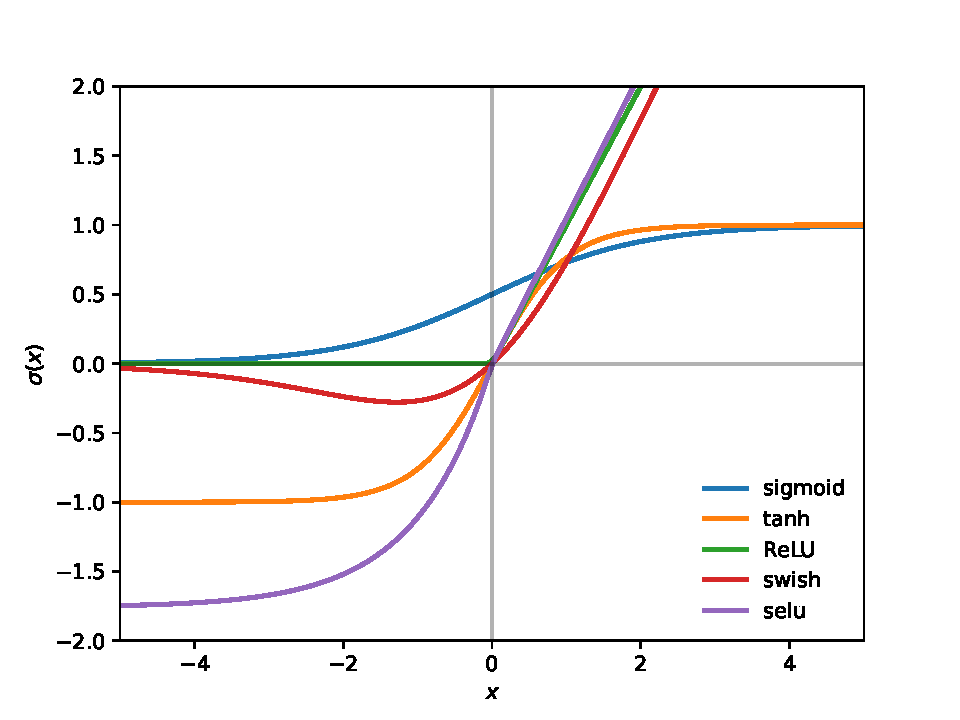
\includegraphics[trim={0cm 0cm 0cm 0cm},clip]{activations.pdf}}
    \end{figure}

\end{frame}


\begin{frame}{Training}
    
    \begin{figure}
       \centering
       \scalebox{0.54}{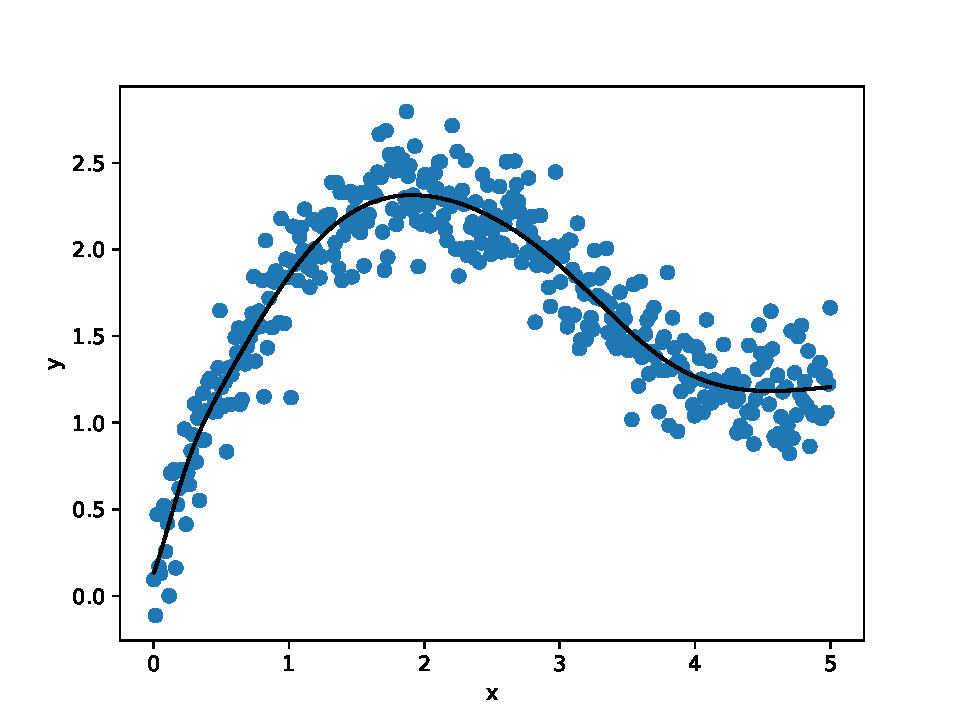
\includegraphics[trim={0cm 0cm 0cm 0cm},clip]{fit_func.pdf}}
    \end{figure}

\end{frame}


\begin{frame}
    
    Aim: Learn to predict output $y$ from input $x$
    %
    \begin{itemize}
        \item $x \in \RR^k$
        \vspace{0.5em}
        \item $y \in \RR$  (regression problem)
    \end{itemize}

    \Egs
    %
    \begin{itemize}
        \item $x = $ cross section of returns, $y = $ return on oil futures tomorrow
        \vspace{0.5em}
        \item $x = $ weather sensor data, $y = $ max temp tomorrow
    \end{itemize}
        \vspace{0.5em}
        \vspace{0.5em}

    Problem:

    \begin{itemize}
        \item observe $(x_i, y_i)_{i=1}^n$ and seek $f$ such that $y_{n+1}
            \approx f(x_{n+1})$
    \end{itemize}


\end{frame}



\begin{frame}

    Nonlinear regression: choose model $\{f_\theta\}_{\theta \in \Theta}$ and minimize the empirical loss
    %
    \begin{equation*}
        \ell(\theta) := \frac{1}{n}\sum_{i=1}^n (y_i - f_\theta(x_i))^2
        \quad \st \quad \theta \in \Theta
    \end{equation*}


    \pause
    \vspace{0.5em}
    In the case of ANNs, we consider all $f_\theta$ having the form
    %
    \begin{equation*}
        f_\theta
        = G_{m} \circ G_{m-1} \circ \cdots \circ G_{2}  \circ G_{1}
    \end{equation*}
    %
    where
    %
    \begin{itemize}
        \item $G_{\ell} x = \sigma_\ell(x W_\ell + b_\ell)$ 
        \vspace{0.5em}
        \item $\sigma_\ell$ is an activation function
    \end{itemize}

\end{frame}

\begin{frame}

    Minimizing the loss functions  
    
    \begin{figure}
       \begin{center}
        \scalebox{0.15}{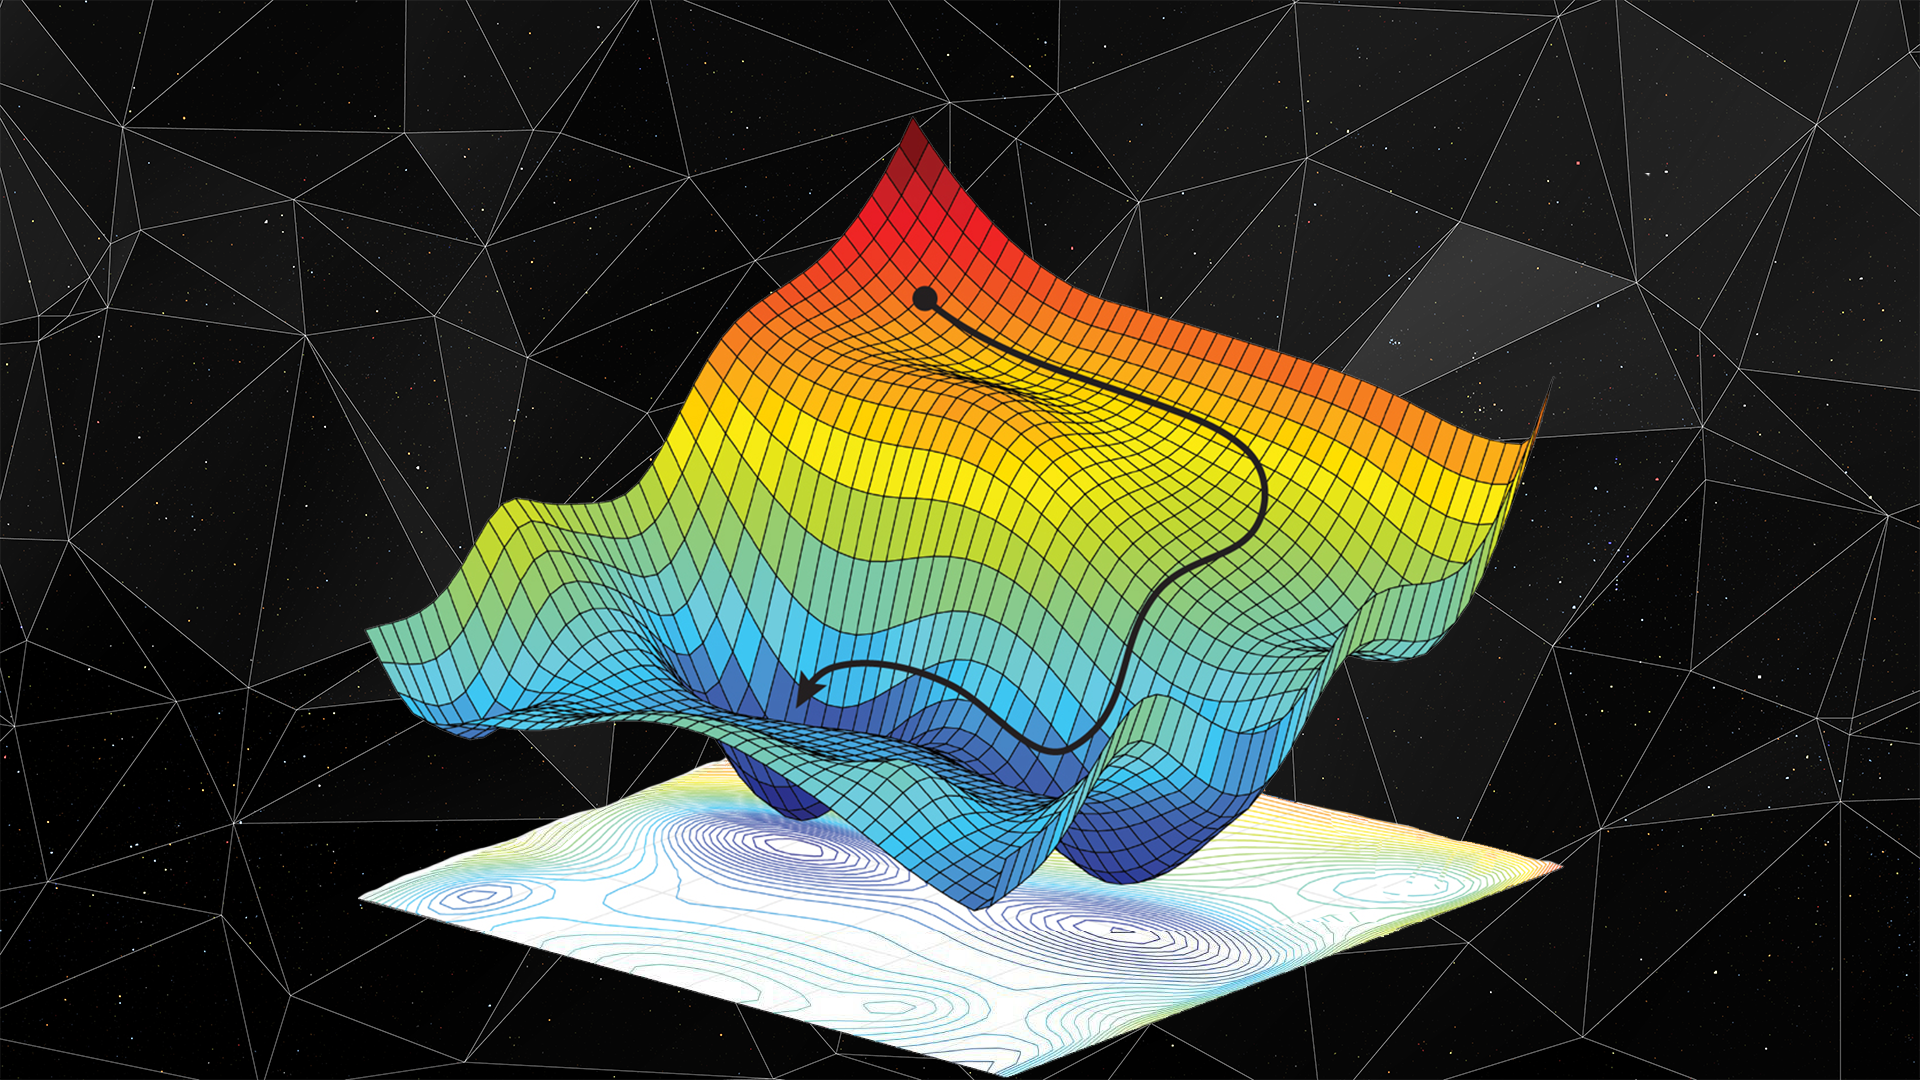
\includegraphics[trim={0cm 0cm 0cm 0cm},clip]{gdi.png}}
       \end{center}
    \end{figure}

    Source: \url{https://danielkhv.com/}

\end{frame}


\begin{frame}{Gradient descent}

    Algorithm:
    
    \begin{equation*}
        \theta_{\rm{next}} = \theta - \lambda \, \nabla_\theta \ell(\theta, x, y)
    \end{equation*}

    \begin{itemize}
        \item take a step in the opposite direction to the grad vector
        \vspace{0.5em}
        \item $\lambda$ is the \emp{learning rate} -- often changes at each step
        \vspace{0.5em}
        \item iterate until hit a stopping condition
        \vspace{0.5em}
        \item in practice replace $\ell(\theta)$ with batched loss
            %
            \begin{equation*}
                \frac{1}{|B|}\sum_{i \in B} (y_i - f_\theta(x_i))^2
            \end{equation*}
    \end{itemize}

    Using batches $\to$ \emp{stochastic gradient descent}

\end{frame}


\begin{frame}{Extensions}


    \begin{itemize}
        \item Loss functions with regularization
        \vspace{0.5em}
        \item Cross-entropy loss (classification)
        \vspace{0.5em}
        \item Convolutional neural networks (image processing)
        \vspace{0.5em}
        \item Recurrent neural networks (sequential data)
        \vspace{0.5em}
        \item Transformers (LLMs)
        \vspace{0.5em}
        \item etc.
    \end{itemize}
    
\end{frame}



\begin{frame}{A mystery}
    
    What about overfitting?

\end{frame}

\begin{frame}
    
    \begin{figure}
       \centering
       \scalebox{0.3}{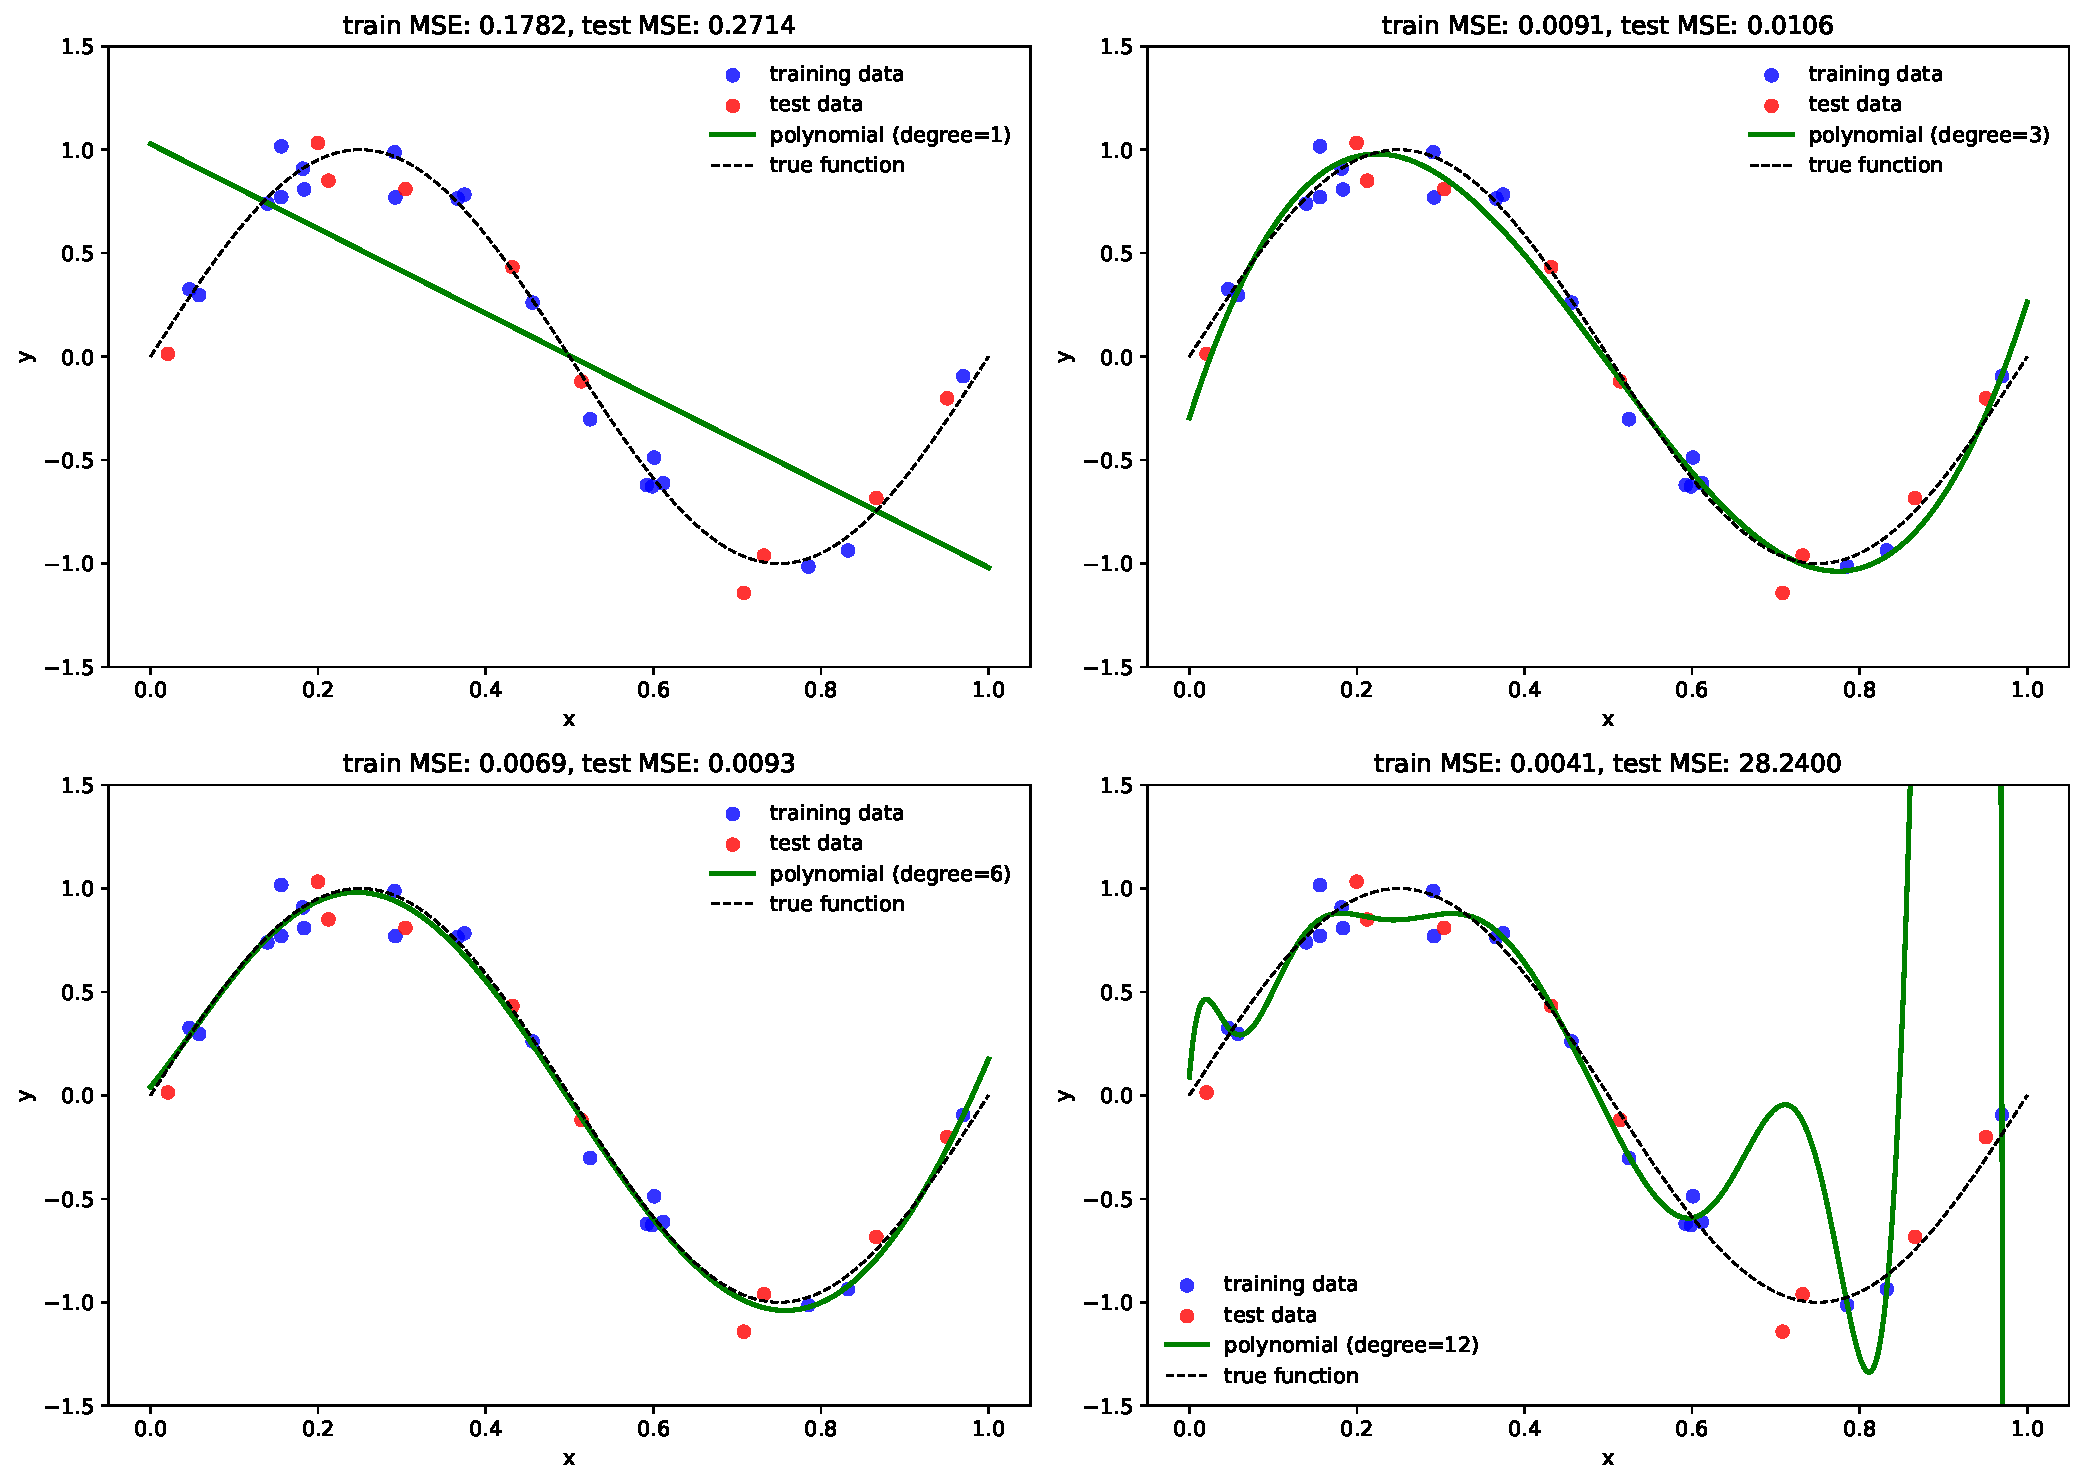
\includegraphics[trim={0cm 0cm 0cm 0cm},clip]{overfit.pdf}}
    \end{figure}

\end{frame}

\begin{frame}
    
    \begin{tikzpicture}
    \begin{axis}[
        width=10cm,
        height=6.6cm,
        xlabel={model complexity},
        ylabel={loss},
        xmin=0, xmax=10,
        ymin=0, ymax=1,
        xticklabels={,,,,,,,,,,},
        yticklabels={,,,,,},
        ylabel near ticks,
        xlabel near ticks,
        legend style={at={(0.97,0.03)}, anchor=south east, draw=none, fill=white, fill opacity=0.7, text opacity=1},
        grid=both,
        grid style={line width=.1pt, draw=gray!10},
        major grid style={line width=.2pt,draw=gray!50},
        every axis plot/.append style={thick},
        title={Overfitting and underfitting},
        title style={font=\large},
        domain=0:10,
        smooth,
    ]

    % Training error curve (monotonically decreasing)
    \addplot[color=blue, line width=2pt, name path=training] {0.9*exp(-0.35*x) + 0.1};

    % Test error curve (U-shaped)
    \addplot[color=red, line width=2pt, name path=test] {0.4*exp(-0.7*x) + 0.15*exp(0.35*(x-5)) + 0.12};

    % curve labels
    \node[color=blue, font=\small\bfseries] at (8,0.25) {training loss};
    \node[color=red, font=\small\bfseries] at (7,0.65) {test loss};

    % Underfitting and overfitting regions
    \draw[<->, >=stealth, gray, line width=1pt] (3.2,0.8) -- (0.2,0.8);
    \node[align=center, gray, font=\small\bfseries] at (1.9, 0.9) {underfitting};

    \draw[<->, >=stealth, gray, line width=1pt] (6.3,0.8) -- (9.8,0.8);
    \node[align=center, gray, font=\small\bfseries] at (8, 0.9) {overfitting};

    % Fill regions
    \path[name path=axis] (axis cs:0,0) -- (axis cs:10,0);
    \addplot[blue!10, opacity=0.5] fill between[of=axis and training, soft clip={domain=0:3.2}];
    \addplot[red!10, opacity=0.5] fill between[of=axis and test, soft clip={domain=3.2:10}];

    \end{axis}

    \end{tikzpicture}

\end{frame}


\begin{frame}
    
    If production-level DL models are so large, why don't they overfit?

        \vspace{0.5em}
        \vspace{0.5em}
        \vspace{0.5em}

    \textbf{Answer 1} Data sets are large and complex -- need complex model

        \vspace{0.5em}
        \vspace{0.5em}
    \textbf{Answer 2} Engineers avoid using full complexity of the model

    \begin{itemize}
        \item Early stopping halts training when test loss starts to rise
        \vspace{0.5em}
        \item Drop out -- shut down some neurons during training
    \end{itemize}


\end{frame}

\begin{frame}
    
    \textbf{Answer 3} Adding randomization to training prevents overfitting

    \begin{itemize}
        \item Related to benefits of random dropout (randomization)
        \vspace{0.5em}
        \item Related techniques in DL such as DropConnect and Stochastic Depth
        \vspace{0.5em}
        \item Stochastic gradient descent injects randomness
    \end{itemize}

        \vspace{0.5em}
        \vspace{0.5em}

    Randomness ``adds some smoothing'' to a given data set

    ``The model must learn to be robust to these perturbations, which encourages
    it to find smoother, more generalizable decision boundaries rather than
    fitting to noise in the training data.'' 



\end{frame}


\begin{frame}
    
    \textbf{Answer 4} Modern architectures have inductive biases that guide
    learning toward useful patterns

    \begin{itemize}
        \item translation invariance in CNNs (same pattern can be
            recognized anywhere in an image)
        \item localization in CNNs -- pixels are influenced more by neighbors
            than pixels far away
        \item parameter sharing in RNNs -- similarity of transformations across
            time
        \item Layer normalization and residual connections in transformers -
            create a bias toward stable training dynamics and information preservation across layers.
    \end{itemize}
    
\end{frame}


\begin{frame}
    
    Finally, there is some evidence of ``double descent'' -- test error starts to fall again
    when the number of parameters is very high

\end{frame}


\begin{frame}
    
    \begin{tikzpicture}
    \begin{axis}[
        width=10cm,
        height=7cm,
        xlabel={number of parameters},
        ylabel={loss},
        xmin=0, xmax=15,
        ymin=0, ymax=1.2,
        xtick={2.5,7.5,12.5},
        xticklabels={low, med, high},
        ytick={0,0.2,0.4,0.6,0.8,1.0,1.2},
        ylabel near ticks,
        xlabel near ticks,
        legend style={at={(0.97,0.03)}, anchor=south east, draw=none, fill=white, fill opacity=0.8},
        grid=major,
        grid style={line width=.2pt, draw=gray!30},
        every axis plot/.append style={thick},
        title={Double descent phenomenon},
        title style={font=\large},
        domain=0:15,
        smooth,
    ]

    % Define interpolation threshold with vertical line
    \addplot[dashed, black, line width=1pt] coordinates {(7.5, 0) (7.5, 1.2)};
    \node[align=center, text width=3cm, font=\small] at (9.5, 1.1) {interpolation threshold};

    % Training error curve
    \addplot[color=blue, line width=2pt] coordinates {
        (0, 1.0)
        (2, 0.7)
        (4, 0.45)
        (6, 0.25)
        (7, 0.1)
        (7.5, 0.02)
        (8, 0.015)
        (10, 0.01)
        (15, 0.005)
    };

    % Test error with double descent
    \addplot[color=red, line width=2pt] coordinates {
        (0, 1.0)
        (2, 0.7)
        (4, 0.4)
        (6, 0.3)
        (7, 0.35)
        (7.5, 0.9)
        (8, 0.7)
        (9, 0.5)
        (11, 0.28)
        (13, 0.2)
        (15, 0.3)
    };

    % Labels
    \node[color=blue, font=\small\bfseries] at (12,0.1) {training loss};
    \node[color=red, font=\small\bfseries] at (12,0.4) {test loss};


    \end{axis}
    \end{tikzpicture}

\end{frame}




\begin{frame}{Summary}
    
    Why can deep learning successfully generalize from limited observations?

\end{frame}


\begin{frame}{Computer scientists' story}

    \begin{itemize}
        \item Good because based on a model of the human brain! 
        \vspace{0.5em}
        \vspace{0.5em}
        \item A universal function approximator!
        \vspace{0.5em}
        \vspace{0.5em}
        \item Can break the curse of dimensionality!
    \end{itemize}


\end{frame}

\begin{frame}{Alternative story (me)}


    \begin{itemize}
        \item A highly flexible function fitting technique 
        \vspace{0.5em}
        \item Easy to understand with limited maths background
        \vspace{0.5em}
        \item Extends naturally to high dimensions 
        \vspace{0.5em}
        \item Can exploit low-dimensional structure
        \vspace{0.5em}
        \item Function evaluations are highly parallelizable
        \vspace{0.5em}
        \item Smooth recursive structure suited to calculating gradients
        \vspace{0.5em}
        \item Has received \underline{massive} investment from the CS community
            \begin{itemize}
                \vspace{0.5em}
                \item algos, software, hardware
            \end{itemize}
    \end{itemize}

\end{frame}

\begin{frame}
    
    \begin{itemize}
        \vspace{0.5em}
        \item Many incremental improvements to improve regularization and training
        \vspace{0.5em}
        \item Many incremental improvements to inject domain-specific knowledge
            (CNNs, transformers, etc.)
    \end{itemize}

\end{frame}

\end{document}


